\documentclass[t]{beamer}
\usepackage{physics}
\usepackage{amsmath}
\usepackage{tikz}
\usepackage{mathdots}
\usepackage{yhmath}
\usepackage{cancel}
\usepackage{color}
\usepackage{siunitx}
\usepackage{array}
\usepackage{multirow}
\usepackage[version=4]{mhchem}
\usepackage{amssymb}
\usepackage{textcomp, gensymb}
\usepackage{mathtools}
\usepackage{pifont}
\newcommand{\cmark}{\ding{51}}%
\newcommand{\xmark}{\ding{55}}%
\usepackage{tabularx}
\usepackage{extarrows}
\usepackage{booktabs}
\usetikzlibrary{fadings}
\usetikzlibrary{patterns}
\usetikzlibrary{shadows.blur}
\usetikzlibrary{shapes}
\usepackage[style=authoryear,backend=bibtex]{biblatex}
\addbibresource{gw.bib}
\renewcommand{\footnotesize}{\scriptsize}
\usepackage{listings}
\usepackage{hyperref}

\newcommand{\pair}[1]{\langle #1 \rangle}
\DeclareMathOperator{\ee}{e}
\DeclareMathOperator{\ii}{i}
\DeclareMathOperator{\sgn}{sgn}

\newcommand{\concept}[1]{\textbf{#1}}
\newcommand*{\abinitio}{\textit{ab initio}}
\newcommand{\shortcode}[1]{\texttt{#1}}

%region Theme 

\usetheme{madrid}

% Show section in foot
\makeatletter
\setbeamertemplate{footline}
{
  \leavevmode%
  \hbox{%
  \begin{beamercolorbox}[wd=.333333\paperwidth,ht=2.25ex,dp=1ex,center]{author in head/foot}%
    \usebeamerfont{author in head/foot}\insertauthor
  \end{beamercolorbox}%
  \begin{beamercolorbox}[wd=.333333\paperwidth,ht=2.25ex,dp=1ex,center]{title in head/foot}%
    \usebeamerfont{title in head/foot}\insertsection
  \end{beamercolorbox}%
  \begin{beamercolorbox}[wd=.333333\paperwidth,ht=2.25ex,dp=1ex,right]{date in head/foot}%
    \usebeamerfont{date in head/foot}\insertshortdate{}\hspace*{2em}
    \insertframenumber{} / \inserttotalframenumber\hspace*{2ex} 
  \end{beamercolorbox}}%
  \vskip0pt%
}
\makeatother

%endregion

%Information to be included in the title page:
\title{Details in $GW$-BSE}
\author{Jinyuan Wu}

\begin{document}

\maketitle

\begin{frame}
    \frametitle{Table of contents}

    \tableofcontents

\end{frame}

\section{The theory}

\begin{frame}
\frametitle{Infinitesimal}

We all know the word ``$GW$'' means that $\Sigma = \ii G W$ 
(of course we have Hartree term but it's already in DFT)

\begin{equation}
    \protect- \ii \Sigma =\tikzset{every picture/.style={line width=0.75pt}} %set default line width to 0.75pt        
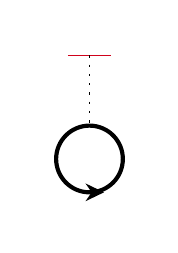
\begin{tikzpicture}[x=0.75pt,y=0.75pt,yscale=-1,xscale=1, baseline=(XXXX.south) ]
\path (0,95);\path (58.66667175292969,0);\draw    ($(current bounding box.center)+(0,0.3em)$) node [anchor=south] (XXXX) {};
%Straight Lines [id:da3194897839790105] 
\draw [color={rgb, 255:red, 208; green, 2; blue, 27 }  ,draw opacity=1 ]   (19.33,13.33) -- (29.78,13.33) ;
%Straight Lines [id:da9155294698759933] 
\draw [color={rgb, 255:red, 208; green, 2; blue, 27 }  ,draw opacity=1 ]   (29.78,13.33) -- (40.23,13.33) ;
%Straight Lines [id:da13142497560962174] 
\draw  [dash pattern={on 0.84pt off 2.51pt}]  (29.78,13.33) -- (29.78,47.19) ;
%Shape: Circle [id:dp8962966421220611] 
\draw  [color={rgb, 255:red, 0; green, 0; blue, 0 }  ,draw opacity=1 ][line width=1.5]  (13.71,63.26) .. controls (13.71,54.38) and (20.9,47.19) .. (29.78,47.19) .. controls (38.66,47.19) and (45.85,54.38) .. (45.85,63.26) .. controls (45.85,72.14) and (38.66,79.33) .. (29.78,79.33) .. controls (20.9,79.33) and (13.71,72.14) .. (13.71,63.26) -- cycle ;
%Straight Lines [id:da7168487847478093] 
\draw [color={rgb, 255:red, 0; green, 0; blue, 0 }  ,draw opacity=1 ]   (29.78,79.33) -- (33.78,79.33) ;
\draw [shift={(36.78,79.33)}, rotate = 180] [fill={rgb, 255:red, 0; green, 0; blue, 0 }  ,fill opacity=1 ][line width=0.08]  [draw opacity=0] (8.93,-4.29) -- (0,0) -- (8.93,4.29) -- (5.93,0) -- cycle    ;
\end{tikzpicture}
+\tikzset{every picture/.style={line width=0.75pt}} %set default line width to 0.75pt        
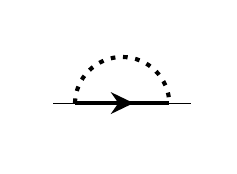
\begin{tikzpicture}[x=0.75pt,y=0.75pt,yscale=-1,xscale=1, baseline=(XXXX.south) ]
\path (0,57);\path (87.33333587646484,0);\draw    ($(current bounding box.center)+(0,0.3em)$) node [anchor=south] (XXXX) {};
%Straight Lines [id:da4779610823231175] 
\draw [color={rgb, 255:red, 0; green, 0; blue, 0 }  ,draw opacity=1 ]   (12.33,36.33) -- (22.78,36.33) ;
%Straight Lines [id:da9873503675232067] 
\draw [color={rgb, 255:red, 0; green, 0; blue, 0 }  ,draw opacity=1 ]   (68.1,36.33) -- (78.55,36.33) ;
%Straight Lines [id:da09313351721820862] 
\draw [color={rgb, 255:red, 0; green, 0; blue, 0 }  ,draw opacity=1 ][line width=1.5]    (22.78,36.33) -- (68.1,36.33) ;
\draw [shift={(51.04,36.33)}, rotate = 180] [fill={rgb, 255:red, 0; green, 0; blue, 0 }  ,fill opacity=1 ][line width=0.08]  [draw opacity=0] (11.07,-5.32) -- (0,0) -- (11.07,5.32) -- (7.35,0) -- cycle    ;
%Shape: Arc [id:dp7767262671888671] 
\draw  [draw opacity=0][dash pattern={on 1.69pt off 2.76pt}][line width=1.5]  (22.78,36.33) .. controls (23.05,23.96) and (33.2,14.05) .. (45.62,14.11) .. controls (58.08,14.17) and (68.16,24.25) .. (68.24,36.67) -- (45.51,36.84) -- cycle ; \draw  [color={rgb, 255:red, 0; green, 0; blue, 0 }  ,draw opacity=1 ][dash pattern={on 1.69pt off 2.76pt}][line width=1.5]  (22.78,36.33) .. controls (23.05,23.96) and (33.2,14.05) .. (45.62,14.11) .. controls (58.08,14.17) and (68.16,24.25) .. (68.24,36.67) ;  
\end{tikzpicture},
\end{equation}
where $W$ is the RPA-screened potential.

\vspace{0.25cm}
\textbf{Why some say $\Sigma(1, 2) = \ii G(1, 2) W(1^+, 2)$?}

\begin{itemize}
    \item $G(1, 2)$ is actually $G(1, 2^+)$ (so when $1=2$, $G = n_{\text{occ}}$: 
    the loop in the Hartree term above)
    \item $\Sigma(1, 2) = \ii G(1, 2^+) W(1, 2) = \ii G(1^-, 2) W(1, 2) = \ii G(1, 2) (1^+, 2)$.
    \item $1^+$ or $2^+$ $\Leftrightarrow$ $\ee^{\pm \ii \omega 0^+}$
        $\Leftrightarrow$ how to take contour 
\end{itemize}

\end{frame}

\begin{frame}
\frametitle{Other tricky details in diagrammatics}

\textbf{Time-reversal symmetry}

\begin{itemize}
    \item $W(- \vb*{p} , -\omega) = W(\vb*{p}, \omega)$ is always true 
        (or otherwise we can symmetrize the Lagrangian)
    \item The real symmetry: 
    \begin{equation}
        \begin{aligned}
            &W(\omega, -\vb*{k}) = W(\omega, \vb*{k}) \Leftrightarrow 
            W(- \omega, \vb*{k}) = W(\omega, \vb*{k})  \\
            \Leftrightarrow &W(\vb*{r}, \vb*{r}', \omega) = W(\vb*{r}', \vb*{r}, \omega) \Leftrightarrow
            W(\vb*{r}, \vb*{r}', \omega) = W(\vb*{r}, \vb*{r}', - \omega).
        \end{aligned}
    \end{equation}
\end{itemize}

\textbf{``Antiparticles''} You can treat holes as antiparticles 
(negative energy, $\ii \sgn(\xi_{n \vb*{k}})$ in time-ordered Green function)
but then corresponding electron modes have to be ignored. 

\end{frame}

\begin{frame}
\frametitle{Other tricky details in diagrammatics}

\textbf{Imaginary unit} 
\begin{equation}
    \protect\ii G= \ii G_{0} + \ii G_{0} \times 
\underbrace{
    \begin{gathered}
        \tikzset{every picture/.style={line width=0.75pt}} %set default line width to 0.75pt        
        \begin{tikzpicture}[x=0.75pt,y=0.75pt,yscale=-0.6,xscale=0.6, baseline=(XXXX.south) ]
            %\path (0,75);\path (56,0);\draw    ($(current bounding box.center)+(0,0.3em)$) node [anchor=south] (XXXX) {};
            %Shape: Circle [id:dp046942194255674474] 
            \draw  [fill={rgb, 255:red, 155; green, 155; blue, 155 }  ,fill opacity=1 ] (8.54,37.54) .. controls (8.54,27.35) and (16.81,19.08) .. (27,19.08) .. controls (37.19,19.08) and (45.46,27.35) .. (45.46,37.54) .. controls (45.46,47.74) and (37.19,56) .. (27,56) .. controls (16.81,56) and (8.54,47.74) .. (8.54,37.54) -- cycle ;
        \end{tikzpicture}
    \end{gathered}
}_{- \ii \Sigma} \times \ii G
    \Rightarrow G = \frac{1}{\omega - E^0 - \Sigma}.
\end{equation}    
\begin{equation}
    \protect- \ii W = - \ii v + (- \ii v) \times 
\underbrace{
    \begin{gathered}
        \tikzset{every picture/.style={line width=0.75pt}} %set default line width to 0.75pt        
        \begin{tikzpicture}[x=0.75pt,y=0.75pt,yscale=-0.6,xscale=0.6, baseline=(XXXX.south) ]
            %\path (0,75);\path (56,0);\draw    ($(current bounding box.center)+(0,0.3em)$) node [anchor=south] (XXXX) {};
            %Shape: Circle [id:dp046942194255674474] 
            \draw  [fill={rgb, 255:red, 155; green, 155; blue, 155 }  ,fill opacity=1 ] (8.54,37.54) .. controls (8.54,27.35) and (16.81,19.08) .. (27,19.08) .. controls (37.19,19.08) and (45.46,27.35) .. (45.46,37.54) .. controls (45.46,47.74) and (37.19,56) .. (27,56) .. controls (16.81,56) and (8.54,47.74) .. (8.54,37.54) -- cycle ;
        \end{tikzpicture}
    \end{gathered}
}_{ \ii \chi} \times (- \ii W)
    \Rightarrow W = \epsilon^{-1} v, \quad \epsilon = 1 - v \chi.
\end{equation}

\textbf{Minus sign} 

Note that when a closed fermionic loop is formed, 
a $-1$ factor is needed. Example: the loop in the Hartree term
$\simeq (-1) \expval{\psi \psi^\dagger} \simeq \psi^\dagger \psi \simeq \text{number of particle}$.

\end{frame}

\begin{frame}[allowframebreaks]
\frametitle{Feynman rules}

Recall that we are working in a crystal -- we need to talk about $\vb*{G}$ vectors

One set of rules that work: 
\begin{itemize}
    \item Propagator: \begin{equation}
        \begin{gathered}
            \begin{tikzpicture}[x=0.75pt,y=0.75pt,yscale=-1,xscale=1, baseline=(XXXX.south) ]
                \path (0,57);\path (86,0);\draw    ($(current bounding box.center)+(0,0.3em)$) node [anchor=south] (XXXX) {};
                %Straight Lines [id:da8778734653821205] 
                \draw    (5,30) -- (76.5,30) ;
                \draw [shift={(44.55,30)}, rotate = 180] [fill={rgb, 255:red, 0; green, 0; blue, 0 }  ][line width=0.08]  [draw opacity=0] (8.93,-4.29) -- (0,0) -- (8.93,4.29) -- (5.93,0) -- cycle    ;
                % Text Node
                \draw (40.75,23.5) node [anchor=south] [inner sep=0.75pt]    {$n,k$};
                \end{tikzpicture}
        \end{gathered} =
        \frac{\ii}{\omega - \xi_{n\vb*{k}} + \ii 0^+ \sgn(\omega)} \eqqcolon \ii G^0_{n \vb*{k}}(\omega).
    \end{equation}
    \item Interaction: 
    \begin{equation}
        \begin{gathered}
            \begin{tikzpicture}[x=0.75pt,y=0.75pt,yscale=-1,xscale=1, baseline=(XXXX.south) ]
                \path (0,57);\path (86,0);\draw    ($(current bounding box.center)+(0,0.3em)$) node [anchor=south] (XXXX) {};
                %Straight Lines [id:da7824913889732596] 
                \draw  [dash pattern={on 0.84pt off 2.51pt}]  (5,30) -- (76.5,30) ;
                % Text Node
                \draw (40.75,23.5) node [anchor=south] [inner sep=0.75pt]    {$q,\vb*{G}$};
            \end{tikzpicture}
        \end{gathered} =
        - \ii \frac{1}{V} v(\vb*{q} + \vb*{G}).
    \end{equation}
    But the prefactor of the interaction Hamiltonian is still $1/2V$, and 
    \begin{equation}
        v(\vb*{q}) = \int \dd[3]{\vb*{r}} \ee^{- \ii \vb*{q} \cdot \vb*{r}} v(\vb*{r}).
    \end{equation}
    \item For vertex, 
    \begin{equation}
        \begin{gathered}
            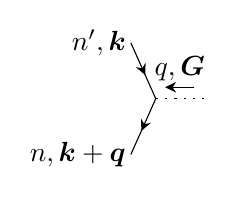
\begin{tikzpicture}[x=0.75pt,y=0.75pt,yscale=-0.6,xscale=0.6]
                %uncomment if require: \path (0,162); %set diagram left start at 0, and has height of 162
                
                %Straight Lines [id:da200203398607687] 
                \draw    (45.5,27.33) -- (65.5,72.17) ;
                \draw [shift={(57.05,53.22)}, rotate = 245.96] [fill={rgb, 255:red, 0; green, 0; blue, 0 }  ][line width=0.08]  [draw opacity=0] (8.93,-4.29) -- (0,0) -- (8.93,4.29) -- (5.93,0) -- cycle    ;
                %Straight Lines [id:da642061936562244] 
                \draw    (65.5,72.17) -- (45.5,117) ;
                \draw [shift={(53.95,98.05)}, rotate = 294.04] [fill={rgb, 255:red, 0; green, 0; blue, 0 }  ][line width=0.08]  [draw opacity=0] (8.93,-4.29) -- (0,0) -- (8.93,4.29) -- (5.93,0) -- cycle    ;
                %Straight Lines [id:da4169224489697443] 
                \draw  [dash pattern={on 0.84pt off 2.51pt}]  (65.5,72.17) -- (105.5,72.17) ;
                %Straight Lines [id:da035273687574558066] 
                \draw    (76,63) -- (96.5,63) ;
                \draw [shift={(73,63)}, rotate = 0] [fill={rgb, 255:red, 0; green, 0; blue, 0 }  ][line width=0.08]  [draw opacity=0] (8.93,-4.29) -- (0,0) -- (8.93,4.29) -- (5.93,0) -- cycle    ;
                
                % Text Node
                \draw (84.75,60) node [anchor=south] [inner sep=0.75pt]    {$q, \vb*{G}$};
                % Text Node
                \draw (43.5,27.33) node [anchor=east] [inner sep=0.75pt]    {$n', \vb*{k}$};
                % Text Node
                \draw (43.5,117) node [anchor=east] [inner sep=0.75pt]    {$n, \vb*{k}+\vb*{q}$};
                \end{tikzpicture}                
        \end{gathered} = 
        \mel{n, \vb*{k} + \vb*{q}}{\ee^{\ii (\vb*{q} + \vb*{G}) \cdot \vb*{r}}}{n' \vb*{k}}
        \eqqcolon M_{n n'} (\vb*{k}, \vb*{q}, \vb*{G}) .
        \label{eq:m-def}
    \end{equation}
    Note that the momentum arrow attached to the interaction line only controls 
    the sign before $\vb*{q}$ and $\vb*{G}$; 
    we don't sum over possible directions of the arrow. 
    Thus 
    \begin{equation}
        \begin{gathered}
            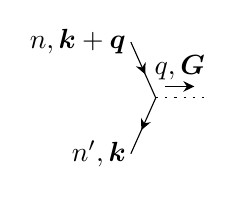
\begin{tikzpicture}[x=0.75pt,y=0.75pt,yscale=-0.6,xscale=0.6]
                %uncomment if require: \path (0,162); %set diagram left start at 0, and has height of 162
                
                %Straight Lines [id:da200203398607687] 
                \draw    (45.5,27.33) -- (65.5,72.17) ;
                \draw [shift={(57.05,53.22)}, rotate = 245.96] [fill={rgb, 255:red, 0; green, 0; blue, 0 }  ][line width=0.08]  [draw opacity=0] (8.93,-4.29) -- (0,0) -- (8.93,4.29) -- (5.93,0) -- cycle    ;
                %Straight Lines [id:da642061936562244] 
                \draw    (65.5,72.17) -- (45.5,117) ;
                \draw [shift={(53.95,98.05)}, rotate = 294.04] [fill={rgb, 255:red, 0; green, 0; blue, 0 }  ][line width=0.08]  [draw opacity=0] (8.93,-4.29) -- (0,0) -- (8.93,4.29) -- (5.93,0) -- cycle    ;
                %Straight Lines [id:da4169224489697443] 
                \draw  [dash pattern={on 0.84pt off 2.51pt}]  (65.5,72.17) -- (105.5,72.17) ;
                %Straight Lines [id:da035273687574558066] 
                \draw    (73,63) -- (93.5,63) ;
                \draw [shift={(96.5,63)}, rotate = 180] [fill={rgb, 255:red, 0; green, 0; blue, 0 }  ][line width=0.08]  [draw opacity=0] (8.93,-4.29) -- (0,0) -- (8.93,4.29) -- (5.93,0) -- cycle    ;
                
                % Text Node
                \draw (84.75,60) node [anchor=south] [inner sep=0.75pt]    {$q, \vb*{G}$};
                % Text Node
                \draw (43.5,27.33) node [anchor=east] [inner sep=0.75pt]    {$n, \vb*{k} + \vb*{q}$};
                % Text Node
                \draw (43.5,117) node [anchor=east] [inner sep=0.75pt]    {$n', \vb*{k}$};
                \end{tikzpicture}
        \end{gathered} = \mel{n' \vb*{k}}{\ee^{- \ii (\vb*{q} + \vb*{G}) \cdot \vb*{r}}}{n, \vb*{k} + \vb*{q}}
        \eqqcolon M_{n n'}(\vb*{k}, \vb*{q}, \vb*{G})^* .
    \end{equation}

    Here is where the phase factor of each $\phi_{n \vb*{k}}$ enters the calculation: 
    
    \item Momentum conservation is enforced by 
    $\delta_{\vb*{k}_1 + \vb*{k}_2 + \vb*{k}_3 + \vb*{k}_4, 0}$:
    no $(2\pi)^3$ factor is needed. 

    \item For internal lines, 
    sum over $\vb*{k}, n, \vb*{G}$; no additional $1 / (2\pi)^3$ factors are needed. 
    For frequency, do $\int \dd{\omega} / 2 \pi$.
    \item For external lines:
        $
        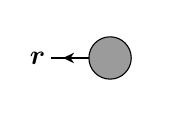
\begin{tikzpicture}[x=0.75pt,y=0.75pt,yscale=-0.6,xscale=0.6, baseline=(XXXX.south) ]
            \path (0,49);\path (95,0);\draw    ($(current bounding box.center)+(0,0.3em)$) node [anchor=south] (XXXX) {};
            %Straight Lines [id:da6811482684267909] 
            \draw    (18.33,24.33) -- (49.17,24.33) ;
            \draw [shift={(28.45,24.33)}, rotate = 0] [fill={rgb, 255:red, 0; green, 0; blue, 0 }  ][line width=0.08]  [draw opacity=0] (8.93,-4.29) -- (0,0) -- (8.93,4.29) -- (5.93,0) -- cycle    ;
            %Shape: Circle [id:dp1659562467053013] 
            \draw  [fill={rgb, 255:red, 155; green, 155; blue, 155 }  ,fill opacity=1 ] (49.17,24.33) .. controls (49.17,14.94) and (56.78,7.33) .. (66.17,7.33) .. controls (75.56,7.33) and (83.17,14.94) .. (83.17,24.33) .. controls (83.17,33.72) and (75.56,41.33) .. (66.17,41.33) .. controls (56.78,41.33) and (49.17,33.72) .. (49.17,24.33) -- cycle ;
            % Text Node
            \draw (16.33,24.33) node [anchor=east] [inner sep=0.75pt]    {$\boldsymbol{r}$};
            \end{tikzpicture}$ is $\phi_{n \vb*{k}}(\vb*{r})$, and 
        $
        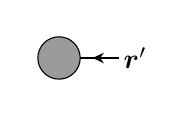
\begin{tikzpicture}[x=0.75pt,y=0.75pt,yscale=-0.6,xscale=0.6, baseline=(XXXX.south) ]
        \path (0,49);\path (95,0);\draw    ($(current bounding box.center)+(0,0.3em)$) node [anchor=south] (XXXX) {};
        %Straight Lines [id:da7875336501425136] 
        \draw    (42.17,24.33) -- (73,24.33) ;
        \draw [shift={(52.28,24.33)}, rotate = 0] [fill={rgb, 255:red, 0; green, 0; blue, 0 }  ][line width=0.08]  [draw opacity=0] (8.93,-4.29) -- (0,0) -- (8.93,4.29) -- (5.93,0) -- cycle    ;
        %Shape: Circle [id:dp7005939415994358] 
        \draw  [fill={rgb, 255:red, 155; green, 155; blue, 155 }  ,fill opacity=1 ] (8.17,24.33) .. controls (8.17,14.94) and (15.78,7.33) .. (25.17,7.33) .. controls (34.56,7.33) and (42.17,14.94) .. (42.17,24.33) .. controls (42.17,33.72) and (34.56,41.33) .. (25.17,41.33) .. controls (15.78,41.33) and (8.17,33.72) .. (8.17,24.33) -- cycle ;
        % Text Node
        \draw (75,24.33) node [anchor=west] [inner sep=0.75pt]    {$\boldsymbol{r} '$};
        \end{tikzpicture}$ is $\phi^*_{n \vb*{k}}(\vb*{r})$, as in: 
        \begin{equation}
            G(\vb*{r}, \vb*{r}', \omega) = \sum_{n, \vb*{k}}
            \frac{\phi_{n \vb*{k}}(\vb*{r}) \phi_{n \vb*{k}}(\vb*{r}')^*}{\omega - \xi_{n \vb*{k}} 
            + \ii \sgn(\xi_{n \vb*{k}})} ,
        \end{equation}
        where $\vb*{r}$ is the outgoing index and $\vb*{r}'$ is the incoming index.
        (When going from $G(\vb*{r}, \vb*{r}')$ to $G_{\vb*{k}, nn'}$, 
        outgoing external line becomes $\phi^*_{n\vb*{k}}(\vb*{r})^*$
        and incoming external line becomes $\phi_{n' \vb*{k}}(\vb*{r}')$)

        The normalization condition is 
        \begin{equation}
            \int \dd[3]{\vb*{r}} \psi^*_{n \vb*{k}} (\vb*{r}) \psi_{n' \vb*{k}'}(\vb*{r})
            = \delta_{n n'} \delta_{\vb*{k} \vb*{k}'}, \quad 
            \psi_{n \vb*{k}} \simeq \frac{1}{\sqrt{V}} \ee^{\ii (\vb*{k} + \vb*{G}) \cdot \vb*{r}}.
        \end{equation}
\end{itemize}

\end{frame}

\section{$GW$ without $G$}

\begin{frame}
\frametitle{The structure of $G$}

\begin{itemize}
    \item We \emph{always} have Lehmann self-energy representations:
    \begin{equation}
        G(\vb*{r}, \vb*{r}', \omega) = \sum_n \frac{
            \mel{\Omega}{\phi(\vb*{r})}{n} \mel{n}{\phi^\dagger(\vb*{r}')}{\Omega}
        }{
            \omega - E_n + \ii 0^+ \sgn(\omega)
        }  
        = \sum_{n, \vb*{k}} 
        \frac{\phi_{n \vb*{k}}(\vb*{r}) \phi_{n \vb*{k}}(\vb*{r}')^*}{
            \omega - \Re \xi_{n \vb*{k}} - \ii \Im \xi_{n \vb*{k}}
        }.
    \end{equation}
    $\vb*{k}$ not necessarily good quantum number; 
    no orthogonal conditions. 
    \item In a Fermi liquid: since $\tau \propto 1 / T^2$ near $\mu$, 
    for bands near the Fermi surface, 
    approximately $\Im \xi_{n \vb*{k}}$ is small and $\{\phi_{n \vb*{k}}\}$ is a good basis. 
    \item Note: this only means $\ket*{\Omega}$ and $\ket*{n}$ look like 
        Fock states when tested with $G^{(2)}$ 
        (hence clear-cut $\mu$ in simulated ARPES spectrum, etc.); 
        when tested with $G^{(4)}$, correlated effects still exist 
        ($\Rightarrow$ de-excitation terms in exciton $\chi_S(\vb*{r}, \vb*{r}')$) 
\end{itemize}

\end{frame}

\begin{frame}
\frametitle{The structure of $G$}

To avoid directly dealing with poles numerically 
(and getting stuck by things like how small $\ii 0^+$ should really be), 
we choose to carry out $\ii GW$ analytically. 

\textbf{Assumption: well-defined quasiparticles} So we assume 
\begin{equation}
    G(\vb*{r}, \vb*{r}', \omega) 
    = \sum_{n, \vb*{k}} \frac{
        \phi_{n \vb*{k}}(\vb*{r}) \phi_{n \vb*{k}}^*(\vb*{r}')
    }{
        \omega - \xi_{n \vb*{k}} + \ii \sgn(\xi_{n \vb*{k}})
    }.
\end{equation}

\textbf{Spectral function} \begin{equation}
    A(\vb*{r}, \vb*{r}', \omega)
    = \sum_{n, \vb*{k}} \delta(\omega - \xi_{n \vb*{k}})
    \phi_{n \vb*{k}}(\vb*{r}) \phi^*_{n \vb*{k}}(\vb*{r}').
\end{equation}


\end{frame}

\begin{frame}
\frametitle{The structure of $W$}

\textbf{Time reversal symmetry} We assume
\begin{equation}
    W(\vb*{r}, \vb*{r}', \omega) = W(\vb*{r}, \vb*{r}', - \omega).
\end{equation}

\textbf{The explicit expression in terms of $\phi_{n \vb*{k}}$} (The $-1$ factor comes from the fermion loop)

\begin{equation}
    \begin{aligned}
        \ii \chi_{\vb*{G} \vb*{G}'}(\vb*{q}, \omega) &= 
        \begin{gathered}
            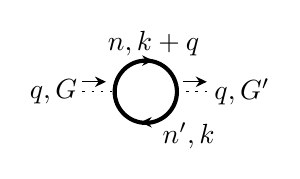
\begin{tikzpicture}[x=0.75pt,y=0.75pt,yscale=-0.6,xscale=0.6]
                %uncomment if require: \path (0,106); %set diagram left start at 0, and has height of 106
                
                %Shape: Circle [id:dp21973504133666855] 
                \draw  [line width=1.5]  (63.51,59) .. controls (63.51,45.19) and (74.7,34) .. (88.51,34) .. controls (102.32,34) and (113.51,45.19) .. (113.51,59) .. controls (113.51,72.81) and (102.32,84) .. (88.51,84) .. controls (74.7,84) and (63.51,72.81) .. (63.51,59) -- cycle ;
                %Straight Lines [id:da37559817089176883] 
                \draw    (88.51,34) -- (91.39,34) ;
                \draw [shift={(94.39,34)}, rotate = 180] [fill={rgb, 255:red, 0; green, 0; blue, 0 }  ][line width=0.08]  [draw opacity=0] (8.93,-4.29) -- (0,0) -- (8.93,4.29) -- (5.93,0) -- cycle    ;
                %Straight Lines [id:da755691190930156] 
                \draw    (93.64,83.5) -- (87.39,83.5) ;
                \draw [shift={(84.39,83.5)}, rotate = 360] [fill={rgb, 255:red, 0; green, 0; blue, 0 }  ][line width=0.08]  [draw opacity=0] (8.93,-4.29) -- (0,0) -- (8.93,4.29) -- (5.93,0) -- cycle    ;
                %Straight Lines [id:da8734800214005785] 
                \draw  [dash pattern={on 0.84pt off 2.51pt}]  (37.5,59) -- (63.51,59) ;
                %Straight Lines [id:da17683013213779142] 
                \draw  [dash pattern={on 0.84pt off 2.51pt}]  (113.51,59) -- (139.52,59) ;
                %Straight Lines [id:da7454208139341723] 
                \draw    (37.5,51) -- (53.5,51) ;
                \draw [shift={(56.5,51)}, rotate = 180] [fill={rgb, 255:red, 0; green, 0; blue, 0 }  ][line width=0.08]  [draw opacity=0] (8.93,-4.29) -- (0,0) -- (8.93,4.29) -- (5.93,0) -- cycle    ;
                %Straight Lines [id:da8015961496989172] 
                \draw    (118.5,51) -- (134.5,51) ;
                \draw [shift={(137.5,51)}, rotate = 180] [fill={rgb, 255:red, 0; green, 0; blue, 0 }  ][line width=0.08]  [draw opacity=0] (8.93,-4.29) -- (0,0) -- (8.93,4.29) -- (5.93,0) -- cycle    ;
                
                % Text Node
                \draw (35.5,59) node [anchor=east] [inner sep=0.75pt]    {$q,G$};
                % Text Node
                \draw (141.52,59) node [anchor=west] [inner sep=0.75pt]    {$q,G'$};
                % Text Node
                \draw (100,82) node [anchor=north west][inner sep=0.75pt]    {$n',k$};
                % Text Node
                \draw (56,8) node [anchor=north west][inner sep=0.75pt]    {$n,k+q$};
                
                
                \end{tikzpicture}            
        \end{gathered} \\
        &= - \int \frac{\dd{\omega'}}{2\pi} \sum_{\vb*{k}} \sum_{n, n'}
        \frac{\ii}{\omega' - \xi_{n' \vb*{k}} + \ii 0^+ \sgn(\xi_{n' \vb*{k}})} \\
        &\quad \quad \times \frac{\ii}{\omega + \omega' - \xi_{n, \vb*{k} + \vb*{q}} + \ii 0^+ \sgn(\xi_{n, \vb*{k} + \vb*{q}})} \\
        &\quad \quad \times M_{n n' } (\vb*{k}, \vb*{q}, \vb*{G}) M_{nn'}^* (\vb*{k}, \vb*{q}, \vb*{G}') .
    \end{aligned}
\end{equation}

\end{frame}

\begin{frame}
\frametitle{The structure of $W$}

After long and tedious contour integration \dots
\begin{equation}
    \begin{aligned}
        \chi_{\vb*{G} \vb*{G}'}(\vb*{q}, \omega)
        &= \sum_{\vb*{k}} \sum_{n}^{\text{occ}} \sum_{n'}^{\text{emp}} 
        M_{n n'} (\vb*{k}, \vb*{q}, \vb*{G}) M^*_{nn'} (\vb*{k}, \vb*{q}, \vb*{G}') \\
        &\times \left(
        \frac{
            1
        }{
            \omega + \xi_{n, \vb*{k} + \vb*{q}} - \xi_{n' \vb*{k}} + \ii 0^+
        }
        + \frac{
            1
        }{
            - \omega + \xi_{n, \vb*{k} + \vb*{q}} - \xi_{n' \vb*{k}} + \ii 0^+
        }
        \right).
    \end{aligned}
    \label{eq:chi-full}
\end{equation}

Sketch of steps: 
\begin{itemize}
    \item When the signs of $\xi_{n, \vb*{k} + \vb*{q}}$ and $\xi_{n' \vb*{k}}$
        are different, 
        the poles of the two propagators don't cancel.
    \item Time reversal symmetry allows 
        swapping $n$ and $n'$ and adding necessary minus signs to momenta 
    \item So now we can fix $n$ to the occupied band 
        and $n'$ to the empty band 
        and still have the shared $M M^*$ factor for the two terms. 
\end{itemize}

\end{frame}

\begin{frame}[allowframebreaks]
\frametitle{Non-static COHSEX decomposition}

\textbf{Analytic structure of $GW$} Below $\vb*{r}$ and $\vb*{r}'$ indices are hidden;
$\Im$ treats $\phi_{n \vb*{k}}$ as real numbers;
positivity conditions are assumed for 
weight functions in spectral representations:
\begin{equation}
    \Sigma(\omega) = \ii \int \frac{\dd{\omega'}}{2\pi} 
    \ee^{- \ii 0^+ \omega'} G(\omega - \omega') W(\omega') ,
\end{equation}
\begin{equation}
    G(\omega) = \int \dd{\omega'} \frac{A(\omega')}{\omega - \omega' + \ii \sgn(\omega)}, 
    \quad A(\omega) = - \frac{1}{\pi} \abs{\Im G(\omega)},
\end{equation}
\begin{equation}
    W(\omega) = v + \int_{0}^{\infty} \dd{\omega'}
    \frac{2 \omega'}{\omega^2 - (\omega' - \ii 0^+)^2} B(\omega'), \quad 
    \Im W(\omega) = - \pi B(\omega).
\end{equation}

\textbf{The decomposition} So in $G(\omega - \omega')$ and $W(\omega')$
we both have poles \dots
\begin{itemize}
    \item $\Sigma^{\text{COH}}$ = $\Sigma^{GW}$ from poles of $W$ 
    \item $\Sigma^{\text{SEX}}$ = $\Sigma^{GW}$ from poles of $G$
\end{itemize} 

\textbf{Screened exchange term: $\Sigma^{\text{SEX}}$} 

\begin{itemize}
    \item When $\ii \sgn(\omega') < 0$ in $G(\omega)$,
        we have one pole in the lower plane, 
        otherwise no pole exists. 
        We need to integrate on the lower plane 
        (due to $\ee^{- \ii 0^+ \omega'}$ factor). Thus:
        \begin{equation}
            \begin{aligned}
                \Sigma^{\text{SEX}}(\vb*{r}, \vb*{r}', \omega) 
                &= - \int^0_{-\infty} \dd{\omega'} A(\vb*{r}, \vb*{r}', \omega') 
                W(\vb*{r}, \vb*{r}', \omega - \omega') \\
                &= - \sum_{n, \vb*{k}}^{\text{occ}}
                \phi_{n \vb*{k}}(\vb*{r}) \phi_{n \vb*{k}}^*(\vb*{r}') 
                W(\vb*{r}, \vb*{r}', \omega - \xi_{n \vb*{k}}).
            \end{aligned}
        \end{equation}
    \item Inserting the definition of $W$, 
        and switching to the $n, \vb*{k}$ basis: 
        \begin{equation}
            \begin{aligned}
                &\quad \mel{n \vb*{k}}{\Sigma^{\text{SEX}}(\omega)}{n' \vb*{k}} \\
                &= - \sum_{n''}^{\text{occ}} \sum_{\vb*{q} \vb*{G} \vb*{G}'}
                M^*_{n'' n} (\vb*{k}, - \vb*{q}, - \vb*{G}) M_{n'' n'} (\vb*{k}, - \vb*{q},  -\vb*{G}') \\
                &\quad\quad \times  \epsilon^{-1}_{\vb*{G} \vb*{G}'}(\vb*{q}, \omega - \xi_{n'', \vb*{k} - \vb*{q}}) 
                v(\vb*{q} + \vb*{G}') .
            \end{aligned}
            \label{eq:sex}
        \end{equation}
\end{itemize}

\textbf{Comments}

\begin{itemize}
    \item $\Sigma^{\text{SEX}}$ is the only term in Hartree-Fock approx. 
    \item Easy to understand: ``screened repulsive opens the band gap''
\end{itemize}

\framebreak

\textbf{Coulomb hole term: $\Sigma^{\text{COH}}$} 
\begin{itemize}
    \item Consider the poles from $W$, 
        and insert the definition of $A$: 
    \begin{equation}
        \begin{aligned}
            \Sigma^{\text{COH}}(\vb*{r}, \vb*{r}', \omega)
            &= \int_{0}^{\infty} \dd{\omega''} \int_{-\infty}^\infty \dd{\omega'}
            \frac{
                A(\vb*{r}, \vb*{r}', \omega') B(\vb*{r}, \vb*{r}', \omega'')
            }{
                \omega - \omega' - \omega'' + \ii \sgn(\omega')
            } \\ 
            &= \sum_{n, \vb*{k}} \phi_{n \vb*{k}}(\vb*{r}) \phi_{n \vb*{k}}^*(\vb*{r}')
            \int_{0}^{\infty} \dd{\omega'}
            \frac{- \Im W(\vb*{r}, \vb*{r}', \omega') / \pi}{\omega - \xi_{n \vb*{k}} - \omega' + \ii \sgn(\xi_{n \vb*{k}})}.
        \end{aligned}
    \end{equation}
    \item Here the $\epsilon^{-1}$ factor in $W$ 
        is always the same as $\epsilon^{-1}_{\text{r}}$ since $\omega' > 0$.
    \item We can verify (recall that here $\Im$ treats $\phi_{n \vb*{k}}$ as a real number 
    and only considers the positions of the poles)
        \[
            2 \ii \Im \frac{1}{a + b \ii} = \frac{1}{a + b \ii} - \frac{1}{a - b \ii}
            \Rightarrow \Im \epsilon^{-1}(\omega')
            = \frac{1}{2\ii} (\epsilon^{-1}_{\text{r}} - \epsilon^{-1}_{\text{a}}).
        \]
    \item Switching to the $n, \vb*{k}$ basis: 
    \begin{equation}
        \begin{aligned}
            &\quad \mel{n \vb*{k}}{\Sigma^{\text{COH}}(\omega)}{n' \vb*{k}} \\
            &= \frac{\ii}{2\pi} \sum_{n''} \sum_{\vb*{q}, \vb*{G}, \vb*{G}'} 
            M^*_{n'' n} (\vb*{k}, - \vb*{q}, - \vb*{G})  M_{n'' n'} (\vb*{k}, - \vb*{q},  -\vb*{G}') \\
            & \times \int_{0}^{\infty} \dd{\omega'} 
            \frac{
                [\epsilon^{\text{r}}_{\vb*{G} \vb*{G}'}]^{-1} (\vb*{q}, \omega')
                - [\epsilon^{\text{a}}_{\vb*{G} \vb*{G}'}]^{-1} (\vb*{q}, \omega') 
            }{\omega - \xi_{n \vb*{k}} - \omega' + \ii 0^+ \sgn(\xi_{n \vb*{k}})} v(\vb*{q}+\vb*{G}') .
        \end{aligned}
        \label{eq:coh}
    \end{equation}
\end{itemize}

\textbf{Comments} \begin{itemize}
    \item TODO: why the name?
    \item Now we switching back to the normal definition of the operator $\Im$ -- 
        note that 
        \[
            \Im \epsilon_{\text{r}}^{-1} = \frac{1}{2\ii} (\epsilon^{-1}_{\text{r}} - \epsilon^{-1}_{\text{a}}) 
        \]
        is only true for systems with inversion symmetry 
        (real wave function, etc.).
    \item In \cite{berkeleygw}, $\Sigma^{\text{COH}}$ and $\Sigma^{\text{SEX}}$
        are actually the retarded version 
        (note that in \eqref{eq:sex} $\epsilon$ is replaced by $\epsilon_{\text{r}}$,
        and in \eqref{eq:coh}) $\ii \sgn(\xi_{n \vb*{k}}) 0^+$ is replaced by $\ii 0^+$.
\end{itemize}

\end{frame}

\begin{frame}[allowframebreaks]
\frametitle{A brief summary of full frequency, non-diagonal $GW$}

\textbf{Key assumptions} \begin{itemize}
    \item Well-defined quasiparticles labeled by $\vb*{k}$ and $n$
    (Fermi liquid theory; used everywhere)
    \item Time-reversal symmetry (used when deriving $\chi$ and doing spectral representation of $W$)
\end{itemize}

\textbf{Input} $\{\phi_{n \vb*{k}}\}$, $\{\varepsilon_{n \vb*{k}}\}$, 
occupation (from which $\mu$ and hence $\xi_{n \vb*{k}} = \varepsilon_{n \vb*{k}} - \mu$
are decided)

\textbf{Main procedures} \begin{itemize}
    \item \shortcode{epsilon}: input $\{\phi_{n \vb*{k}}\}$ and $\{\varepsilon_{n \vb*{k}}\}$, 
    output $\epsilon^{-1}_{\vb*{G} \vb*{G}'}(\vb*{q}, \omega)$
    \begin{enumerate}
        \item From $\{\phi_{n \vb*{k}}\}$ 
        to $M_{n n'}(\vb*{k}, \vb*{q}, \vb*{G})$ using \eqref{eq:m-def}.
        \item From $\varepsilon_{n \vb*{k}}$ to $\chi_{\vb*{G} \vb*{G}'}(\vb*{q}, \omega)$ using \eqref{eq:chi-full}.
        \item From $\chi$ to $\epsilon$.
        \item Finding $\epsilon^{-1}$.
    \end{enumerate}

    \item \shortcode{sigma}: input $\phi_{n \vb*{k}}$, $V_{\text{xc}}$ and $\epsilon^{-1}_{\vb*{G} \vb*{G}'}(\vb*{q}, \omega)$,
    output $\mel{n \vb*{k}}{\Sigma^GW(E)}{n' \vb*{k}}$ and $\varepsilon_{n \vb*{k}}^{GW}$ 
    \begin{enumerate}
        \item From $\{\phi_{n \vb*{k}}\}$ 
        to $M_{n n'}(\vb*{k}, \vb*{q}, \vb*{G})$ using \eqref{eq:m-def}.
        \item From $M_{n n'}(\vb*{k}, \vb*{q}, \vb*{G})$ to 
        $\mel{n \vb*{k}}{\Sigma^{\text{COH}, \text{SEX}}}{n' \vb*{k}}$
        using TODO 
        \item Finding $Z$ using TODO
    \end{enumerate}
\end{itemize}

\textbf{Cutoff parameters} \begin{itemize}
    \item In $\phi_{n \vb*{k}}$: 
    \begin{itemize}
        \item $N_{\text{bands}}$ (i.e. max $n$), 
        \item $\vb*{k}$-grid density, 
        \item $E_{\text{cut}}$ (i.e. $\vb*{G}$-grid size, i.e. spatial resolution)
    \end{itemize}

    \item In $\epsilon^{-1}_{\vb*{G} \vb*{G}'}(\vb*{q}, \omega)$:
    \begin{itemize}
        \item $\vb*{k}$-grid from $\{\phi_{n \vb*{k}}\}$
        \item $N_{\text{bands}}$ (i.e. max $n$ in summation in \eqref{eq:chi-full}) 
        \item $E_{\text{cut}}$ (used to reduce the $\vb*{G}$-grid in $\{\phi_{n \vb*{k}}\}$, 
        which may be too large)
        \item $\omega$-grid 
    \end{itemize}
\end{itemize}

\end{frame}

\section{Dealing with frequency dependence}

\begin{frame}
\frametitle{Overview}

Three levels of frequency dependence:
\begin{enumerate}
    \item Static COHSEX 
    \item Generalized plasmon-pole model (GPP)
    \item Full frequency
\end{enumerate}    

\end{frame}

\section{Calculating absorption}

\begin{frame}[allowframebreaks]
\frametitle{The expression of $\epsilon_2$}

\begin{itemize}
    \item The SI version: 
    \begin{equation}
        \epsilon_2 \coloneqq \Im \epsilon_{\text{r}} = \frac{\pi e^2}{\omega^2 \epsilon_0 V} 
        \sum_S \abs*{\mel**{S}{\vb*{v} \cdot \vu*{e}}{0}}^2 \delta(\omega - \Omega_S).
    \end{equation}
    \item The Gaussian units version: 
    \begin{equation}
        \epsilon_2 = \frac{4 \pi^2 e^2}{\omega^2  V} 
        \sum_S \abs*{\mel**{S}{\vb*{v} \cdot \vu*{e}}{0}}^2 \delta(\omega - \Omega_S).
    \end{equation}
    The value of $\epsilon$ doesn't change in unit conversion, 
    but $e^2 / \epsilon_0$ should be replaced by $4 \pi e^2$. 
    \item With spin degeneracy we have an additional 2 factor 
    (magnetic field not strong, no mechanism of spin splitting, 
    so the input and output spins are the same)
    \item In Rydberg units, $e^2 = 2$
    \item So with spin degeneracy we have  
    \begin{equation}
        \epsilon_2 = \frac{16 \pi^2 }{\omega^2  V} 
        \sum_S \abs*{\mel**{S}{\vb*{v} \cdot \vu*{e}}{0}}^2 \delta(\omega - \Omega_S),
    \end{equation}
    \item  and without spin degeneracy 
    (or when SOC is strong and the spin index has been incorporated into $S$) we have 
    \begin{equation}
        \epsilon_2 = \frac{8 \pi^2 }{\omega^2  V} 
        \sum_S \abs*{\mel**{S}{\vb*{v} \cdot \vu*{e}}{0}}^2 \delta(\omega - \Omega_S).
    \end{equation}
    \item This is the actual formula used in \shortcode{absp0.f90}.
\end{itemize}

\end{frame}

\section{Building the kernel}

\begin{frame}
\frametitle{Interpolation}

\textbf{Two sources of errors} \begin{itemize}
    \item $\vb*{k}$-grid sampling 
    \item Finite number of bands
    (this can be systematically reduced: 
    for \emph{each} $\vb*{k}$, 
    $\{u_{n \vb*{k}}\}_n$ is a complete basis of 
    the space of possible $u_{n \vb*{k}}$.)
\end{itemize}

\end{frame}



\section{References}

\begin{frame}[allowframebreaks]
\frametitle{References}

\printbibliography

\end{frame}

\end{document}